\subsection{Overview}
\begin{figure}[H]
    \centering
    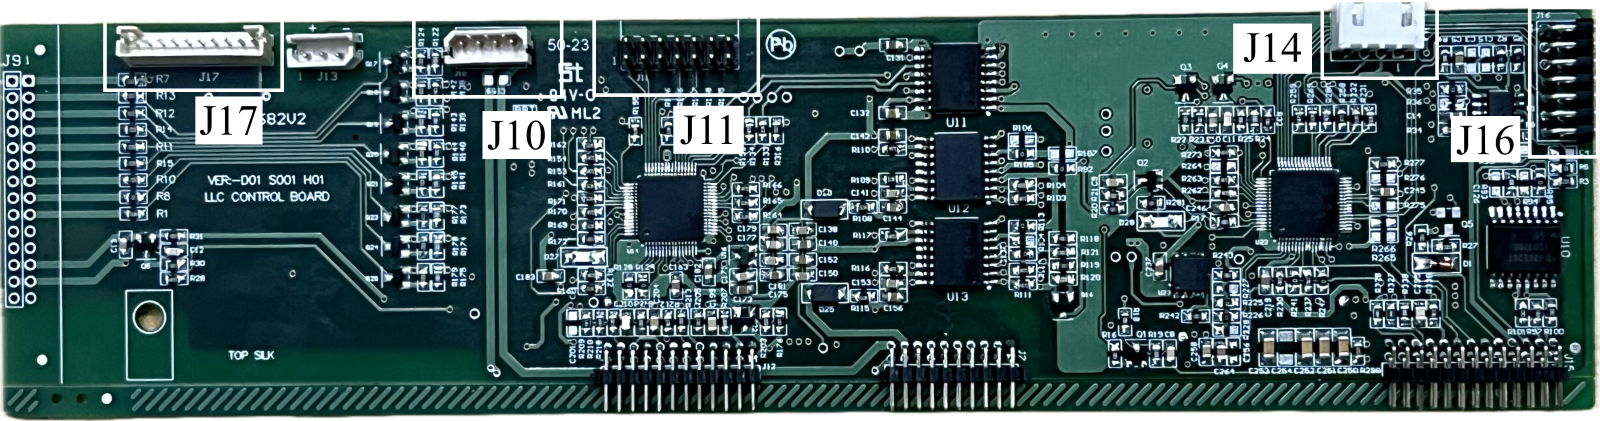
\includegraphics[width=\textwidth]{image9.png}
    \caption{Control Board Circuit}
    \label{fig:image9}
\end{figure}
\begin{itemize}
    \item J10 – Connector for Fan
    \item J11 – Connector for programming the PF
    \item J16 – Connector for programming the LLC
    \item J14 – Connector for debugging (Optional – after complete assembly, J7, RS485 connector on motherboard will be used)
    \item J17 – Connector for Display
\end{itemize}

\subsection{Pre-Testing}

\subsubsection{Safety Equipments}
Wear Safety Equipments such as Insulated Rubber Gloves (Figure \ref{fig:imagea}), and earthing band (Figure \ref{fig:imageb}) before beginning with the testing
\begin{figure}[H]
    \centering
    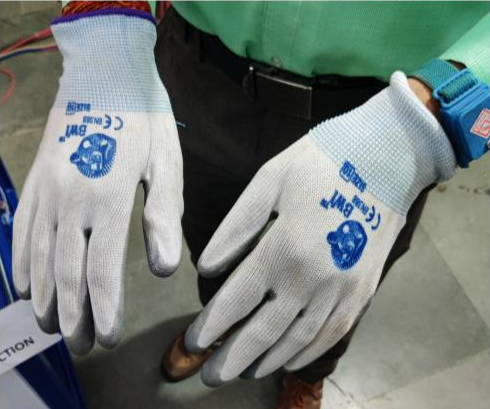
\includegraphics[width=0.5\textwidth]{imagea.png}
    \caption{Insulated Rubber Gloves}
    \label{fig:imagea}
\end{figure}
\begin{figure}[H]
    \centering
    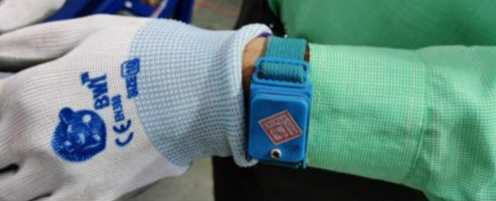
\includegraphics[width=0.5\textwidth]{imageb.png}
    \caption{Earthing Band}
    \label{fig:imageb}
\end{figure}

\subsubsection{Visual Inspection}
The first and foremost part of testing any product involves visually inspecting the PCB to ensure correct component placement as per the schematic and the BOM (Bill of Materials). This also ensures prevention of any physically damaged PCBs to go further the testing line.


\subsection{Control Board Testing}

\subsubsection{Programming the LLC and PFC with Drive-check codes}
\begin{itemize}
    \item Connect J16 to the programmer and upload the LLC drive check code.
    \item Connect J11 to the programmer and upload the PFC drive check code.
\end{itemize}
(Refer to Figure \ref{fig:image9} for the position of the connectors)

\subsubsection{Circuit Connections}
\begin{itemize}
    \item Connect the control card to a tested motherboard as shown in Figure \ref{fig:imagec}.
    \begin{figure}[H]
        \centering
        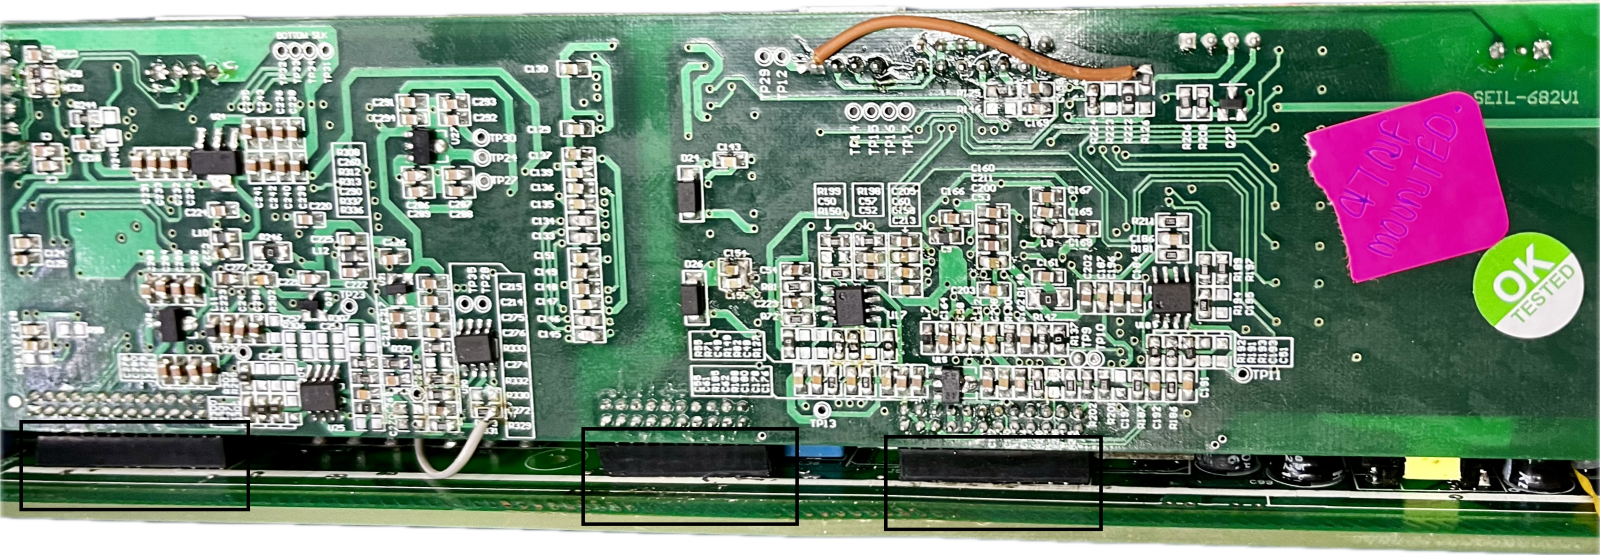
\includegraphics[width=0.6\textwidth]{imagec.png}
        \caption{Headers of the control card to the motherboard}
        \label{fig:imagec}
    \end{figure}
    
    \item Connect the cooling fan to the fan connector at J10 (Figure \ref{fig:imaged}).
    \begin{figure}[H]
        \centering
        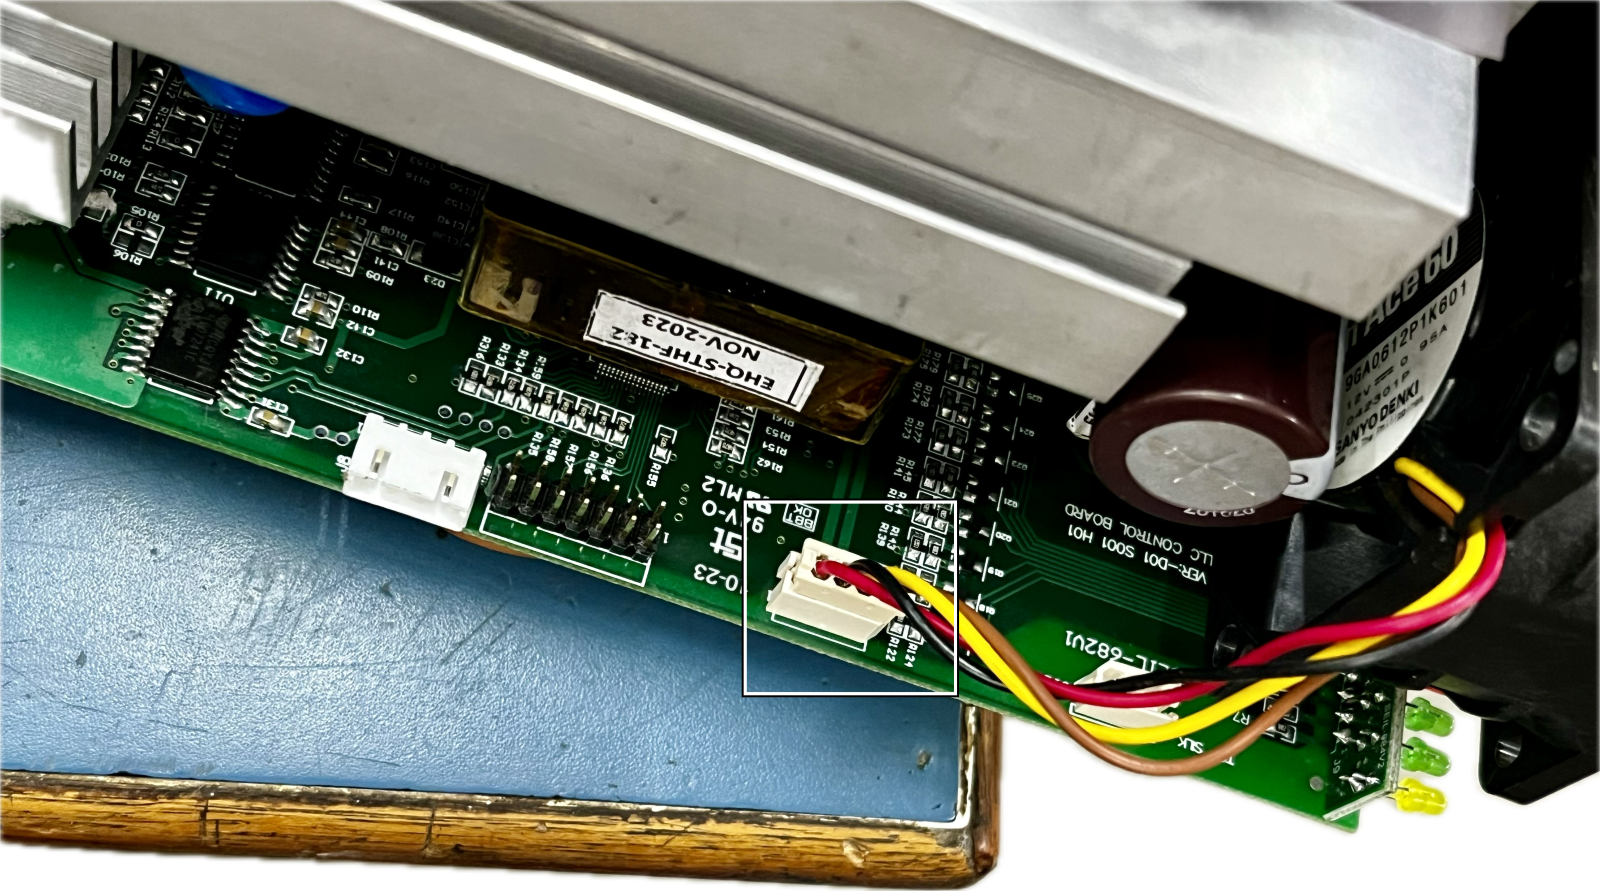
\includegraphics[width=0.5\textwidth]{imaged.png}
        \caption{Fan Connector at J10}
        \label{fig:imaged}
    \end{figure}
    
    \item Ensure no AC supply is connected, and only external DC supply (350-400V) is connected to the motherboard.
    \item Connect display connector (at J17), with one-to-one matching (pin 1 is connected to pin 1, pin 2 to pin 2 and so on... - Figure \ref{fig:image_fan}).
    \begin{figure}[H]
        \centering
        \includegraphics[width=0.3\textwidth, angle=90]{image.jpeg}
        \caption{Display Connector at J17}
        \label{fig:image_fan}
    \end{figure}
\end{itemize}

\subsubsection{Check the Drive (Gate signals at MOSFETs)}
\begin{itemize}
    \item Using an oscilloscope, probe the gate voltages of the MOSFETs of PFC and LLC one-by-one to ensure that all MOSFETs are receiving a PWM signal (square wave type) at their Gate. (probe between 1st and 3rd legs).
\end{itemize}

\subsubsection{Upload Final Code}
\begin{itemize}
    \item Connect J16 to the programmer and upload the LLC final code. 
    \item Connect J11 to the programmer and upload the PFC final code.
    \item Connect laptop to J14 and run mainfile.py. Check that all the measured values are correct. (Such as current – 0A, boost voltage – 0V etc.) - Figure \ref{fig:image10}
\end{itemize}


\subsection{Mother Board Testing}

\subsubsection{Supply Section Check}
\begin{itemize}
    \item Connect an external DC supply (350-400V) to the circuit (At output of PFC - Figure \ref{fig:DC_supply}).
    \begin{figure}[H]
        \centering
        \includegraphics[width=0.2\textwidth]{DC Supply.png}
        \caption{Connecting DC Supply}
        \label{fig:DC_supply}
    \end{figure}
    \item Once it is switched ON, using a multimeter, check the voltages across the following capacitors for confirming the power supply section.
    \begin{itemize}
        \item C113 – 5V (unregulated)
        \item C100 – 12V
        \item C94 – 3.3V
        \item C106 – 12V (unregulated)  
    \end{itemize}
\end{itemize}

\subsubsection{Programming the LLC and PFC with Drive-check codes}
\begin{itemize}
    \item Connect J16 to the programmer and upload the LLC drive check code.
    \item Connect J11 to the programmer and upload the PFC drive check code.
\end{itemize}
(Refer to Figure \ref{fig:image9} for the position of the connectors)

\subsubsection{Circuit Connections}
\begin{itemize}
    \item Connect the tested control card (with drive check code) to the motherboard as shown in Figure \ref{fig:imagec}.
    \item Connect the cooling fan to the fan connector at J10 (Figure \ref{fig:imaged}).
\end{itemize}

\subsubsection{Check the Drive (Gate signals at MOSFETs)}
\begin{itemize}
    \item Using an oscilloscope, probe the gate voltages of the MOSFETs of PFC and LLC one-by-one to ensure that all MOSFETs are receiving a PWM signal (square wave type) at their Gate. (probe between 1st and 3rd legs).
\end{itemize}

\subsubsection{Upload Final Code}
\begin{itemize}
    \item Connect J16 to the programmer and upload the LLC final code. 
    \item Connect J11 to the programmer and upload the PFC final code.
    \item Connect laptop to J14 and run mainfile.py. Check that all the measured values are correct. (Such as current – 0A, boost voltage – 0V etc.) - Figure \ref{fig:image10}
\end{itemize}


\subsection{Assembled Testing}

\subsubsection{Make Final Connections}
\begin{itemize}
    \item Remove DC supply and connect AC supply (150V - 270V RMS) to the motherboard (at J1).
    \item Remove laptop connector at J14.
    \item Connect RS485 connector to J7. 
    \item Connect DSA Comm. connector at J3 (for communication regarding battery charging).
    \item Turn ON the AC Supply.
\end{itemize}

\subsubsection{Run Debugging Tool in Laptop}
\begin{figure}[H]
    \centering
    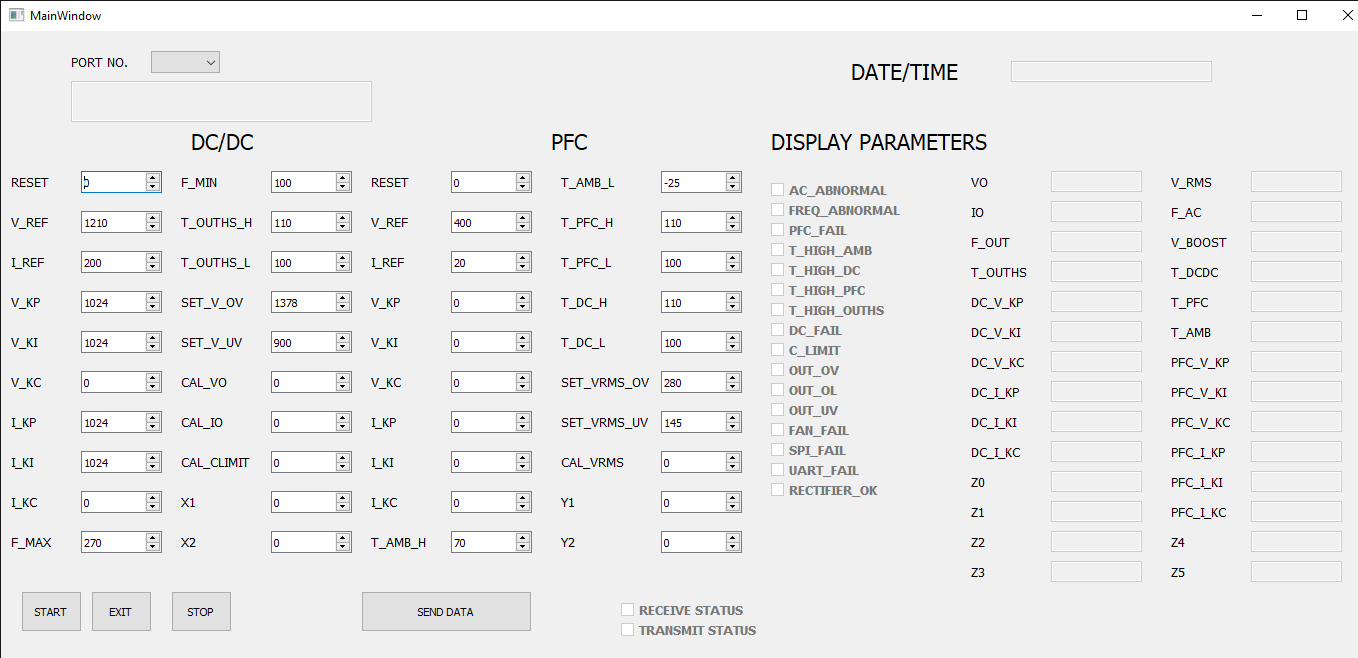
\includegraphics[width=0.6\textwidth]{image10.png}
    \caption{Debugging Tool}
    \label{fig:image10}
\end{figure}
\begin{itemize}
    \item Run mainfile.py on the laptop and then connect it to the motherboard (by pressing START).
    \item Click on SEND DATA.
\end{itemize}

\subsubsection{Verify all functionality}
\begin{itemize}
    \item Verify the data displayed on the screen with the actual readings of the input voltage, output voltage, output current and temperatures to ensure that all feedback mechanisms are working correctly.
    \item Ensure all LEDs are working according to their functions by giving faults (such as giving over voltage at input – 280V RMS, increasing load beyond 20A, when in boost – LED2 will on, etc.)
\end{itemize}